\documentclass{article}
\usepackage{style}
\begin{document}
\maketitle
\part{Introducción}
\section{Neural Networks}

\subsection{Usos principales de las redes neuronales}

Se tienen 4 usos principales de las redes neuronales artificiales (RNA)
\begin{enumerate}
	\item Aproximación de sistemas (Modo regresor)
	\item Predicción de series de tiempo (Modo regresor)
	\item Control de Sistemas (Modo regresor)
	\item Clasificación de objetos (Modo Clasificador)
\end{enumerate}
\subsection{Aproximación de Sistemas}
Dado un sistema $f(t_i)$ del cuál se desconoce su modelo matemático, pero se cuenta con un conjunto de datos entrada-salida $(p, t)$ que representa su comportamiento. Se puede entrenar una RNA para que se comporte de manera similar a $f(t_i)$ en donde:\\\\
$t_i$ : Es la variable de tiempo\\
$p$ : Es la entrada (input)\\
$t$ : El valor deseado (target)\\

\subsection{Modelo Matemático}
Es una representación abstracta que aproxima al comportamiento de un fenómeno real, normalmente mediante un conjunto de ecuaciones.

\subsection{Ecuación}
Igualdad

\subsection{Datos input-output}
Es un conjunto de valores que muestrea mediante sensores el comportamiento dinámico del sistema en todo su rango de funcionamiento

\subsection{Buena Interpolación}
Se llama generación de conocimiento

\subsection{Mala Interpolación}
Se le llama sobrentendimiento

\textbf{LA RED EN MODO REGRESIÓN FUNCIONA COMO UN INTERPOLADOR}

\subsection{Extrapolar}
Pronosticar o predecir, se requieren RNA's recurrentes.

\subsection{Diagrama General}
\begin{figure}[h]
	\caption{Diagrama General}
	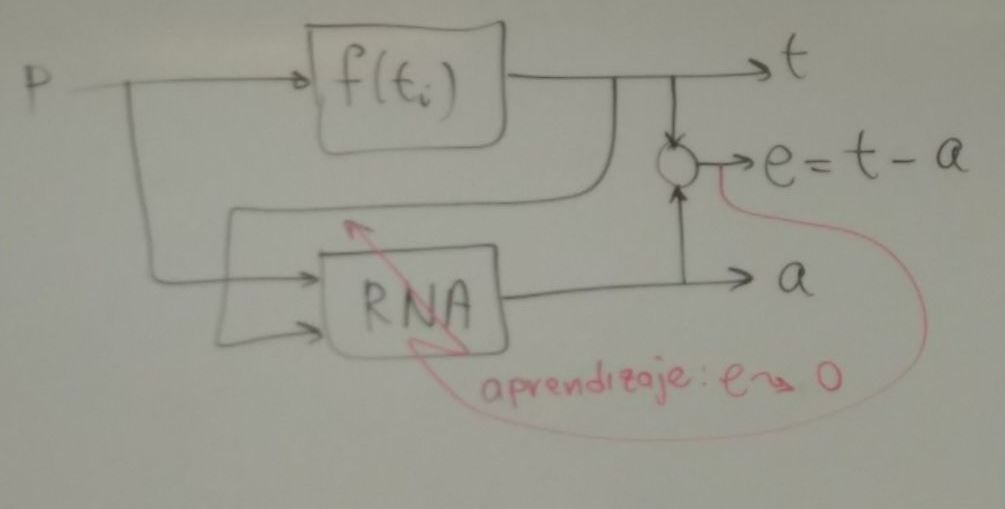
\includegraphics[scale=0.6]{modeloGeneralRn}
\end{figure}

\section{Tipos de Aprendizaje}
\subsection{Aprendizaje Supervisado}
Es aquel en el que se cuenta con ejemplos que contienen valores deseados(target) para llevar a cabo el ajuste de los parámetros de la RNA. En este caso se cuenta con un conjunto de datos$(p, t)$;

\subsection{Aprendizaje no Supervisado}
No se cuenta con ejemplos que contengan valores deseados. Sin embargo, existen diversos algoritmos en esta clasificación que se usan para analizar y extraer información valiosa de una fenómeno, por ejemplo, el algoritmo $k-medias$ recibe como entrada un conjunto de datos y un valor $k$ que representa el número de clases en los que se desea separar a dicho conjunto. Dependiendo del valor de $k$ el usuario podrá analizar de diferentes maneras el fenómeno.

\section{Predicción de Series de tiempo}
Dada una serie de tiempo que representa un fenómeno físico, existe un tiempo especial de RNA que es capaz de pronosticar valores futuros, es decir, realiza la correcta extrapolación de datos. Para esta tarea se hace uso de las RNA's recurrrentes.
\begin{figure}
	\centering
	\caption{Ejemplo de extrapolación}
	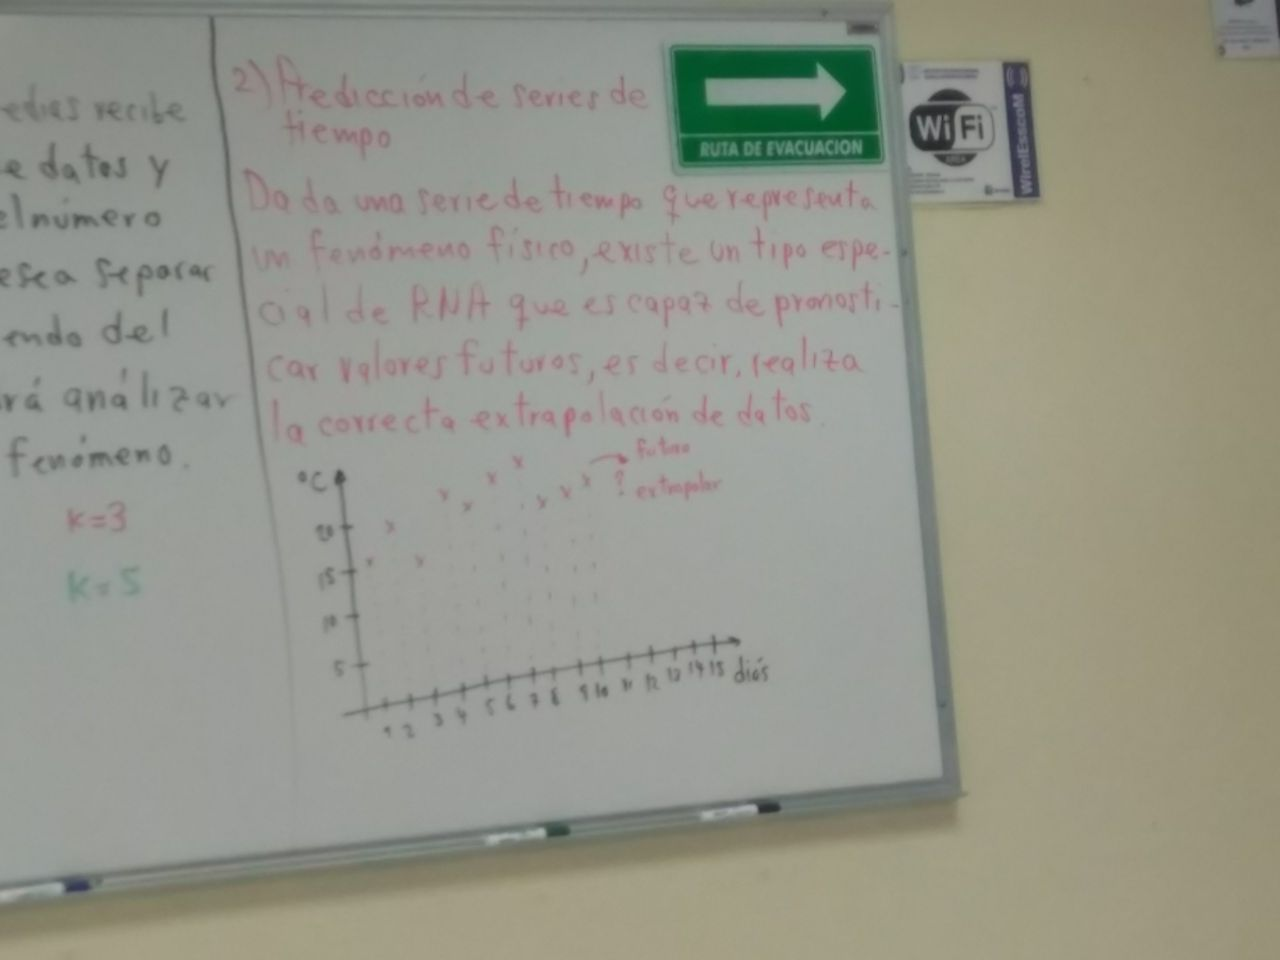
\includegraphics[scale=.4]{exampleTime}	
\end{figure}

\begin{figure}
	\centering
	\caption{Red Feed Foward}
	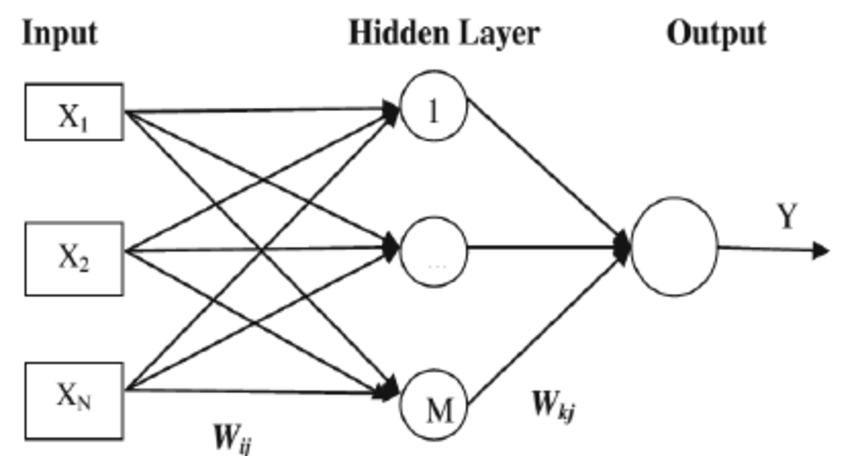
\includegraphics[scale=.5]{feedFowardExample}	
\end{figure}

\begin{figure}
	\centering
	\caption{Red Recurrente}
	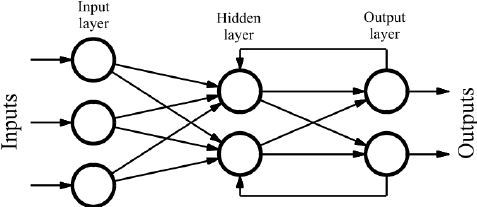
\includegraphics[scale=.8]{recurrentExample}	
\end{figure}

\begin{figure}
	\centering
	\caption{Red Recurrente con bloques recurrentes}
	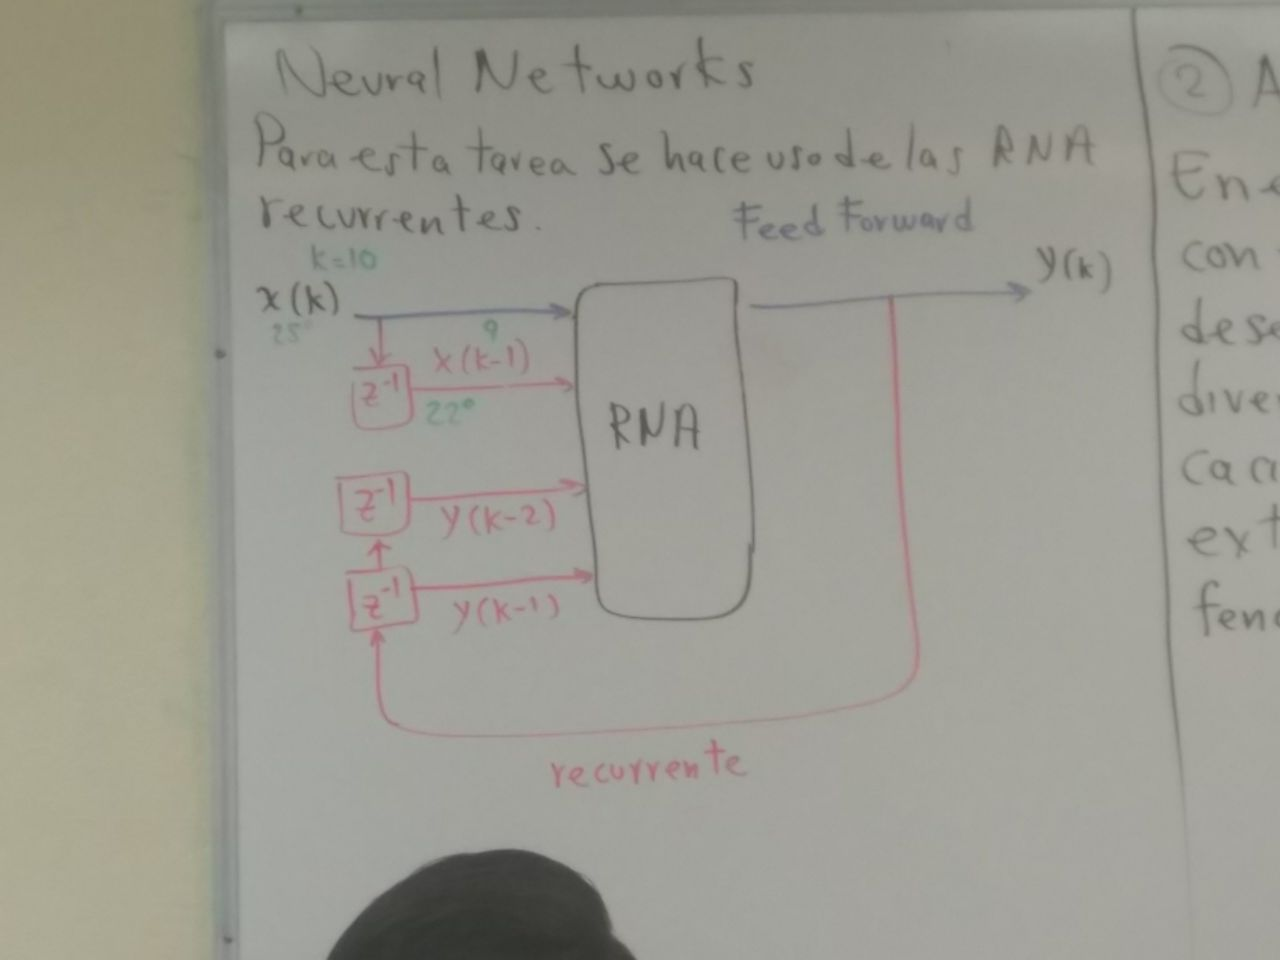
\includegraphics[scale=.37]{recurrentExample2}	
\end{figure}

\section{Control de Sistemas}
Dado un sistema $f(t)$ se requiere modificar su comportamiento para que sea estable. En esta aplicación se usa una RNA para aproximar a $f(t)$ y una RNA para diseñar un controlador.

\begin{figure}
	\centering
	\caption{System Control Example}
	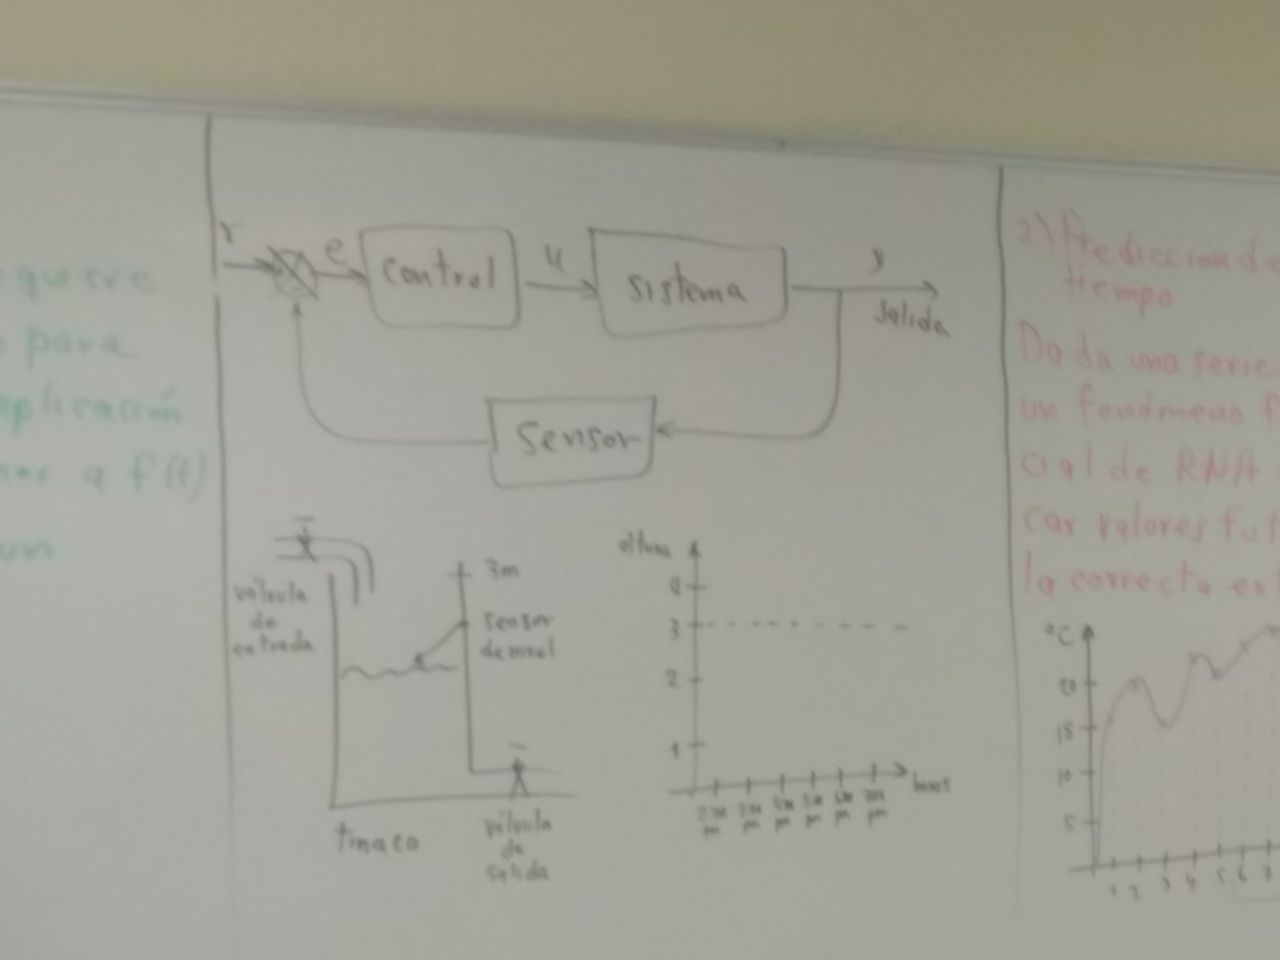
\includegraphics[scale=.37]{systemControlExample1}	
\end{figure}

\end{document}
